\documentclass[11pt,a4paper]{article}
\usepackage[margin=2.3cm]{geometry}
\usepackage[T1]{fontenc}
\usepackage{textcomp}
\input{glyphtounicode}
\pdfgentounicode=1
\usepackage{lmodern}
\usepackage{amsmath}
\usepackage{xcolor}
\usepackage{listings}
\usepackage{tcolorbox}
\usepackage{booktabs}
\usepackage{array}
\usepackage{tikz}
\usepackage{hyperref}
\hypersetup{colorlinks=true, linkcolor=blue!50!black, citecolor=green!40!black}

\usepackage{accsupp}
% line numbers are drawn but excluded from copied text
\newcommand{\nocopy}[1]{\BeginAccSupp{method=escape,ActualText={}}#1\EndAccSupp{}}
\lstset{
  language=C, basicstyle=\ttfamily\small, keywordstyle={}, commentstyle={}, stringstyle={},
  numbers=left, numberstyle=\footnotesize\nocopy, numbersep=10pt, xleftmargin=2.4em,
  frame=none, columns=fullflexible, keepspaces=true, upquote=true, showstringspaces=false,
  breaklines=true, captionpos=b, aboveskip=1em, belowskip=0.8em
}
\lstdefinestyle{sh}{language=bash, numbers=none, xleftmargin=2.4em}
\renewcommand{\lstlistingname}{Listing}
% code names in the text: grey monospace
\let\origtexttt\texttt
\renewcommand{\texttt}[1]{\textcolor{black!60}{\origtexttt{#1}}}

\newtcolorbox{keyidea}{colback=blue!4, colframe=blue!45!black, title=Key ideas, fonttitle=\bfseries\small}
\newtcolorbox{experiment}{colback=orange!5, colframe=orange!70!black, title=Experiment, fonttitle=\bfseries\small}

\title{\textbf{OpenMP Tasks: \texttt{task} and \texttt{taskwait}}\\[4pt]\large Lesson 12: recursive Fibonacci and task granularity}
\author{Gustavo Lozano}
\date{November 2026}

\begin{document}
\maketitle

\noindent\textit{\small Source: van der Pas, Stotzer \& Terboven~\cite{vdp}, chapter on
tasking. Tasks were added in OpenMP~3.0 (2008), after the Chapman book.}

\section{The idea}
Everything so far divided a \emph{loop} (\texttt{for}) or a fixed list of blocks
(\texttt{sections}). Much work has neither shape: recursion, tree and graph traversals,
linked lists, divide-and-conquer algorithms. The number and size of the pieces is only
known while the program runs.

A \textbf{task} is a piece of work, code plus its data, that a thread puts into a
\emph{queue}. Any thread of the team may take it from the queue and execute it, now or
later. One thread can create tasks, and tasks can create more tasks; the idle threads keep
taking them. \texttt{taskwait} makes a task wait until the tasks \emph{it} created
(its children) have finished.

\begin{center}
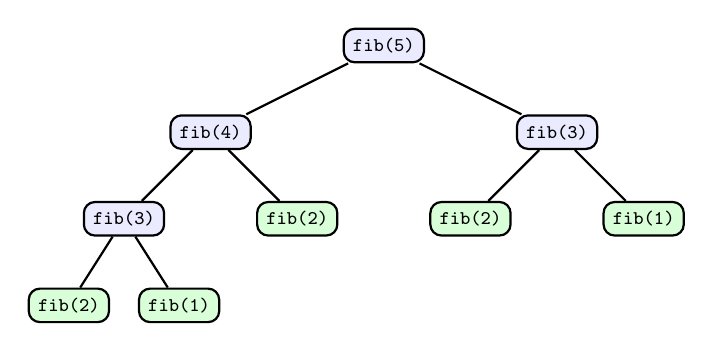
\begin{tikzpicture}[thick, level distance=1.1cm,
  level 1/.style={sibling distance=4.4cm}, level 2/.style={sibling distance=2.2cm},
  level 3/.style={sibling distance=1.4cm},
  every node/.style={draw, rounded corners, font=\scriptsize\ttfamily, fill=blue!8, minimum width=1cm}]
  \node {fib(5)}
    child {node {fib(4)}
      child {node {fib(3)} child {node[fill=green!15] {fib(2)}} child {node[fill=green!15] {fib(1)}}}
      child {node[fill=green!15] {fib(2)}}}
    child {node {fib(3)}
      child {node[fill=green!15] {fib(2)}}
      child {node[fill=green!15] {fib(1)}}};
\end{tikzpicture}

\small \texttt{fib(5)} with cutoff 3. Blue: creates two tasks and waits for them
(\texttt{taskwait}); green: below the cutoff, computed directly without tasks.
\end{center}

\section{The pattern}
\begin{lstlisting}
#pragma omp parallel          /* create the team */
{
    #pragma omp single        /* ONE thread starts the work ...            */
    r = fib(n, cutoff);       /* ... the others execute the tasks it makes */
}                             /* barrier: all tasks are finished here      */
\end{lstlisting}
Inside \texttt{fib}:
\begin{lstlisting}
#pragma omp task shared(a)    /* put "a = fib(n-1)" in the queue */
a = fib(n - 1, cutoff);
#pragma omp task shared(b)    /* put "b = fib(n-2)" in the queue */
b = fib(n - 2, cutoff);
#pragma omp taskwait          /* wait for my two children        */
return a + b;
\end{lstlisting}

\paragraph{Data in tasks.} A task may run after the function that created it has moved on,
so OpenMP gives it a \textbf{copy} of the creating function's local variables:
they are \texttt{firstprivate} by default (Lesson~7). Without \texttt{shared(a)}, the task
would write its result into its own copy of \texttt{a}, which is thrown away, and
\texttt{fib} would return a wrong value (removing both clauses printed
\texttt{fib(30) = 0} in a test).
\texttt{shared(a)} is safe here because \texttt{taskwait} guarantees the task has finished
before \texttt{a} is read, and \texttt{a} still exists at that point.

\paragraph{Granularity.} Creating, queuing and scheduling a task costs time. If a task does
less work than that, tasks make the program \emph{slower}. The \texttt{cutoff} stops creating
tasks for small sub-problems and computes them directly: tasks are created only for
\texttt{n >= cutoff}.

\section{The code}
\lstinputlisting[caption={\textbf{\origtexttt{fib\_tasks.c}} -- recursive Fibonacci with tasks and a cutoff.}]{fib_tasks.c}

\begin{lstlisting}[style=sh]
gcc -Wall -O2 -fopenmp -o fib_tasks fib_tasks.c
OMP_NUM_THREADS=4 ./fib_tasks 42 25
\end{lstlisting}
Output on a 2-core machine (your times will differ):
\begin{lstlisting}[style=sh]
serial : fib(42) = 267914296   0.545 s
tasks  : fib(42) = 267914296   0.339 s   (threads = 2, cutoff = 25, speed-up = 1.61)
\end{lstlisting}

\begin{keyidea}
\begin{itemize}
  \item Tasks parallelize work that is not a loop: one thread creates them, every thread of
        the team executes them.
  \item Use \texttt{parallel} $+$ \texttt{single} to start: one creator, a full team of
        workers.
  \item \texttt{taskwait} waits for the \emph{children} of the current task (not for
        grandchildren; each child waits for its own).
  \item Local variables are \texttt{firstprivate} in a task: results must go to a
        \texttt{shared} variable that lives until the \texttt{taskwait}.
  \item A task must be worth its overhead: use a cutoff.
\end{itemize}
\end{keyidea}

\section{The experiment}
\begin{experiment}
\textbf{Question:} how large should a task be?
\begin{enumerate}
  \item Run \texttt{fib(42)} with all your cores and several cutoffs:
\begin{lstlisting}[style=sh]
export OMP_NUM_THREADS=$(nproc)
for c in 10 15 20 25 30 35 42; do
    ./fib_tasks 42 $c | tail -1
done
\end{lstlisting}
  \item Note the speed-up for each cutoff. The number of tasks each cutoff creates is:
\begin{center}
\small
\begin{tabular}{@{}lrrrrrrr@{}}
\toprule
cutoff & 10 & 15 & 20 & 25 & 30 & 35 & 42 \\ \midrule
tasks created & 18\,454\,928 & 1\,664\,078 & 150\,048 & 13\,528 & 1\,218 & 108 & 2 \\
\bottomrule
\end{tabular}
\end{center}
\end{enumerate}
\textbf{What to observe and answer.}
\begin{enumerate}
  \item With cutoff 10 the parallel version is much \emph{slower} than the serial one. Why?
        Estimate the cost of one task from your times.
  \item With cutoff 42 only 2 tasks are created, \texttt{fib(41)} and \texttt{fib(40)}. What
        is the best speed-up possible, whatever the number of threads?
  \item Which cutoff is best on your machine, and what does it say about the right number of
        tasks compared with the number of threads?
\end{enumerate}
\end{experiment}

\paragraph{Answers (read after trying).}
(1)~Almost every task is tiny: \texttt{fib(10)} takes well under a microsecond, about the
same as creating and scheduling a task. With $1.8\cdot10^7$ tasks the overhead dominates. On
the 2-core test machine cutoff 10 took 11.5\,s against 0.55\,s serial: roughly
$(2\times11.5 - 0.55)\,\text{s} / 1.8\cdot10^7 \approx 1.2\,\mu\text{s}$ of thread time per
task.
(2)~The two tasks are unequal: \texttt{fib(41)} is about 62\% of the work
($\text{fib}(41)/\text{fib}(42) \approx 1/\varphi \approx 0.618$). The run cannot be shorter
than that largest task, so the speed-up is at most $1/0.618 \approx 1.6$, even with 64
threads. Too few tasks means poor load balance.
(3)~Usually a cutoff around 25--35: a few hundred to a few thousand tasks. That is many more
tasks than threads, so idle threads always find work (balance), yet each task is large
enough to hide its overhead. The rule: many more tasks than threads, each much more
expensive than creating it.

\paragraph{Next lesson.} \texttt{taskloop} and task dependencies (\texttt{depend}): ordering
tasks by the data they read and write, without barriers.

\begin{thebibliography}{9}
\bibitem{vdp} R.~van der Pas, E.~Stotzer, and C.~Terboven. \emph{Using OpenMP --- The Next
  Step: Affinity, Accelerators, Tasking, and SIMD}. MIT Press, Cambridge, MA, 2017.
\end{thebibliography}
\end{document}
